\documentclass[12pt,a4paper,]{article}
\usepackage[]{kpfonts}
\usepackage{amssymb,amsmath}
\usepackage{ifxetex,ifluatex}
\usepackage{fixltx2e} % provides \textsubscript
\ifnum 0\ifxetex 1\fi\ifluatex 1\fi=0 % if pdftex
  \usepackage[T1]{fontenc}
  \usepackage[utf8]{inputenc}
\else % if luatex or xelatex
  \ifxetex
    \usepackage{mathspec}
  \else
    \usepackage{fontspec}
  \fi
  \defaultfontfeatures{Ligatures=TeX,Scale=MatchLowercase}
\fi
% use upquote if available, for straight quotes in verbatim environments
\IfFileExists{upquote.sty}{\usepackage{upquote}}{}
% use microtype if available
\IfFileExists{microtype.sty}{%
\usepackage{microtype}
\UseMicrotypeSet[protrusion]{basicmath} % disable protrusion for tt fonts
}{}
\usepackage[margin=1in]{geometry}
\usepackage{hyperref}
\hypersetup{unicode=true,
            pdftitle={Calculating the Housing Wealth Effect of Israeli regional cohorts},
            pdfauthor={Brandon Payne},
            pdfborder={0 0 0},
            breaklinks=true}
\urlstyle{same}  % don't use monospace font for urls
\usepackage[style=authoryear-comp]{biblatex}

\addbibresource{currentEcon.bib}
\usepackage{color}
\usepackage{fancyvrb}
\newcommand{\VerbBar}{|}
\newcommand{\VERB}{\Verb[commandchars=\\\{\}]}
\DefineVerbatimEnvironment{Highlighting}{Verbatim}{commandchars=\\\{\}}
% Add ',fontsize=\small' for more characters per line
\usepackage{framed}
\definecolor{shadecolor}{RGB}{248,248,248}
\newenvironment{Shaded}{\begin{snugshade}}{\end{snugshade}}
\newcommand{\KeywordTok}[1]{\textcolor[rgb]{0.13,0.29,0.53}{\textbf{{#1}}}}
\newcommand{\DataTypeTok}[1]{\textcolor[rgb]{0.13,0.29,0.53}{{#1}}}
\newcommand{\DecValTok}[1]{\textcolor[rgb]{0.00,0.00,0.81}{{#1}}}
\newcommand{\BaseNTok}[1]{\textcolor[rgb]{0.00,0.00,0.81}{{#1}}}
\newcommand{\FloatTok}[1]{\textcolor[rgb]{0.00,0.00,0.81}{{#1}}}
\newcommand{\ConstantTok}[1]{\textcolor[rgb]{0.00,0.00,0.00}{{#1}}}
\newcommand{\CharTok}[1]{\textcolor[rgb]{0.31,0.60,0.02}{{#1}}}
\newcommand{\SpecialCharTok}[1]{\textcolor[rgb]{0.00,0.00,0.00}{{#1}}}
\newcommand{\StringTok}[1]{\textcolor[rgb]{0.31,0.60,0.02}{{#1}}}
\newcommand{\VerbatimStringTok}[1]{\textcolor[rgb]{0.31,0.60,0.02}{{#1}}}
\newcommand{\SpecialStringTok}[1]{\textcolor[rgb]{0.31,0.60,0.02}{{#1}}}
\newcommand{\ImportTok}[1]{{#1}}
\newcommand{\CommentTok}[1]{\textcolor[rgb]{0.56,0.35,0.01}{\textit{{#1}}}}
\newcommand{\DocumentationTok}[1]{\textcolor[rgb]{0.56,0.35,0.01}{\textbf{\textit{{#1}}}}}
\newcommand{\AnnotationTok}[1]{\textcolor[rgb]{0.56,0.35,0.01}{\textbf{\textit{{#1}}}}}
\newcommand{\CommentVarTok}[1]{\textcolor[rgb]{0.56,0.35,0.01}{\textbf{\textit{{#1}}}}}
\newcommand{\OtherTok}[1]{\textcolor[rgb]{0.56,0.35,0.01}{{#1}}}
\newcommand{\FunctionTok}[1]{\textcolor[rgb]{0.00,0.00,0.00}{{#1}}}
\newcommand{\VariableTok}[1]{\textcolor[rgb]{0.00,0.00,0.00}{{#1}}}
\newcommand{\ControlFlowTok}[1]{\textcolor[rgb]{0.13,0.29,0.53}{\textbf{{#1}}}}
\newcommand{\OperatorTok}[1]{\textcolor[rgb]{0.81,0.36,0.00}{\textbf{{#1}}}}
\newcommand{\BuiltInTok}[1]{{#1}}
\newcommand{\ExtensionTok}[1]{{#1}}
\newcommand{\PreprocessorTok}[1]{\textcolor[rgb]{0.56,0.35,0.01}{\textit{{#1}}}}
\newcommand{\AttributeTok}[1]{\textcolor[rgb]{0.77,0.63,0.00}{{#1}}}
\newcommand{\RegionMarkerTok}[1]{{#1}}
\newcommand{\InformationTok}[1]{\textcolor[rgb]{0.56,0.35,0.01}{\textbf{\textit{{#1}}}}}
\newcommand{\WarningTok}[1]{\textcolor[rgb]{0.56,0.35,0.01}{\textbf{\textit{{#1}}}}}
\newcommand{\AlertTok}[1]{\textcolor[rgb]{0.94,0.16,0.16}{{#1}}}
\newcommand{\ErrorTok}[1]{\textcolor[rgb]{0.64,0.00,0.00}{\textbf{{#1}}}}
\newcommand{\NormalTok}[1]{{#1}}
\usepackage{longtable,booktabs}
\usepackage{graphicx,grffile}
\makeatletter
\def\maxwidth{\ifdim\Gin@nat@width>\linewidth\linewidth\else\Gin@nat@width\fi}
\def\maxheight{\ifdim\Gin@nat@height>\textheight\textheight\else\Gin@nat@height\fi}
\makeatother
% Scale images if necessary, so that they will not overflow the page
% margins by default, and it is still possible to overwrite the defaults
% using explicit options in \includegraphics[width, height, ...]{}
\setkeys{Gin}{width=\maxwidth,height=\maxheight,keepaspectratio}
\IfFileExists{parskip.sty}{%
\usepackage{parskip}
}{% else
\setlength{\parindent}{0pt}
\setlength{\parskip}{6pt plus 2pt minus 1pt}
}
\setlength{\emergencystretch}{3em}  % prevent overfull lines
\providecommand{\tightlist}{%
  \setlength{\itemsep}{0pt}\setlength{\parskip}{0pt}}
\setcounter{secnumdepth}{5}

%%% Use protect on footnotes to avoid problems with footnotes in titles
\let\rmarkdownfootnote\footnote%
\def\footnote{\protect\rmarkdownfootnote}

%%% Change title format to be more compact
\usepackage{titling}

% Create subtitle command for use in maketitle
\newcommand{\subtitle}[1]{
  \posttitle{
    \begin{center}\large#1\end{center}
    }
}

\setlength{\droptitle}{-2em}
  \title{Calculating the Housing Wealth Effect of Israeli regional cohorts}
  \pretitle{\vspace{\droptitle}\centering\huge}
  \posttitle{\par}
  \author{Brandon Payne}
  \preauthor{\centering\large\emph}
  \postauthor{\par}
  \date{}
  \predate{}\postdate{}

\usepackage{benyominwp}

% META DATA

\wp{Housing Wealth Effect Proposal}

\jel{C10,C14,C22}

\addresses{
\textbf{Brandon Payne}\\
                Woodman-Scheller Israel Studies International Program\\
                Ben-Gurion University of the Negev\\
                Email: payneb@post.bgu.ac.il\\[1cm]
}

\lfoot{\sf Payne: \Date~\Month~\Year}

\begin{document}
\maketitle

\begin{abstract}
Uses pseudo-panel construction to calculate the housing wealth effect for regional cohorts of Isreali households. Combines data from the Central Bureau of Statistics Household Expenditure Survey and the Consumer Price Index.
\end{abstract}

\begin{keywords}
 consumption, economics, housing, housing market, liquidity constraints, wealth effect 
\end{keywords}

\newpage

\section{Introduction}\label{introduction}

\subsection{The housing market}\label{the-housing-market}

The study of housing provides a fascinating topic for the researcher of
Israeli society. Several factors have drawn attention to the housing
market and made it a topic of much discussion. The price of housing was
one of the main issues that drove more than 400,000 demonstrators to the
streets in the summer of 2011. Large portions of the Israeli population
own a home, or rent one, or live in a multi-family household. Their
first-hand experience of the market may be relayed to the researcher as
anecdotal evidence of the state of the housing market, as well as causes
and solutions for the perceived short-comings of the market.

In a simple economic model of the housing market, house prices are set
by the market forces of supply and demand. Various influences on
suppliers of housing (current owners who choose to sell, builders of new
housing), and those who demand housing (commonly characterized as young
couples) will shift the supply and demand curves and affect the
market-clearing price level. Consider an interest-rate reduction, this
shifts the demand curve to the right, as cheaper credit causes more
buyers to enter the market. It also reduces credit-constraints on
builders and leads to increased supply, albeit after some lag.

The average house price has risen by an astonishing 80\% between the
2008 global financial crisis and 2016. In the minds of many lay
observers this indicates a lack of supply, with main bottlenecks
limiting supply being cited as the sale of government land or the
lengthy permitting process for new construction.

Gruber \autocite{gruberSep2016}, however, offers copious evidence and
cogent reasoning to support his claim that the chief factor in the rise
was actually excessive demand. As global capital markets suffered large
declines investors moved to other asset classes, including the real
estate market. The additional factor of low interest rates lead to a
dramatic increase in purchase of additional houses by those who were
already owner-occupiers. This shifted the demand curve to the right,
increasing the average cost of an apartment and driving out less
affluent first-time homebuyers. These would-be first-time homebuyers
then entered or remained in the rental market, driving up average rents.
The higher market rental prices and lowered vacancy rate established a
feedback loop which further encouraged in the purchase of investment
houses as rental property. \#\# Consumption by Households The
expenditure method for calculating National Income (Y), states that
Y=GDP=C+I+G+NX. The gross domestic product is equal to Consumption
Expenditure (C) plus Investment Expenditure (I) plus Government
Expenditure (G) plus Net Exports (NX). Firms and households each engage
in both consumption and investment. When a firm buys a copy machine
which lasts several years, that is an investment, so is the purchase of
owner-occupied housing, in fact it's one of the chief investments made
by households. The paper placed in the copy machine and the food on the
table are each classified as consumption. Consumption by households
makes up a large and important part of GDP. It is a measure tracked
closely by businesses, economists and the government. You may have heard
the nightly news announce the latest retail-sales data. Household income
is either saved or consumed, with the marginal propensity to consume
(MPC) and the marginal propensity to save (MPS) summing to 1. Generally
household consumption can be understood as household income times the
MPC. The MPC can be affected by the interest rate, rising interest rates
incentivize additional savings, raising the MPS and lowering the MPC.
Falling interest rates decrease the attraction of savings. With a
constant MPC a household can increase consumption due to increased
income from a salary increase, hourly wage increase or increase in the
number of hours worked. Household consumption would fall due a decrease
in salary, wages or working hours. A further factor in consumption is
expected future income. This posits that the rational consumer increases
their consumption now if they know that they will get a raise or some
overtime next week. They will also reduce consumption and increase
savings now when they expect future unemployment or wage reductions.
Another factor affecting consumption is the wealth effect. When the
wealth of a household increases (the price of shares held in an
investment portfolio, the price of Picasso on the wall or in a vault,
the price of the family home or rental property), household consumption
increases, in effect spending now some of the expected future gains on
the sale of the shares, painting or real estate. Conversely, a decline
in household wealth should produce a decline in household consumption
and GDP.

\subsection{Literature Review}\label{literature-review}

\subsubsection{the housing wealth
effect}\label{the-housing-wealth-effect}

Many households around the world store a majority of their wealth in
housing. This, combined with the volatility of swings in house prices,
has caused academics and policy to further investigate the housing
wealth effect and its implications for GDP.\autocite{Gan2010} Renters
and owners should be effected differently by a change in housing prices.
Research using Japanese data showed that renters fell into two
categories when faced with increased housing prices. Some gave up saving
for a housing and instead increased consumption of luxury goods in what
was termed the ``consumption of despair.'' The other group decreased
consumption, and increased their savings rate, still dreaming of home
ownership. These effects on renters were subsequently found in data from
Canada and San Francisco.\autocite{Sheiner_1995} The data used in the
proposed study should allow me to measure the extent to which Israeli
renters engaged in consumption of despair over the last fourteen years.
The life cycle savings hypothesis suggests that consumption of
anticipated increases in wealth will be distributed by consumers over
time, and that there would be a single MPC for both housing wealth and
stock market wealth. When empirically tested, data showed that 85\% of
respondents did not increase consumption in response to a change in
their shares portfolio. Several reasons were suggested why changes in
the value of wealth held in different forms would illicit different
consumption effects from households. Some prices changes in some assets
may be viewed as transitory, others may be harder to measure than the
daily feedback of the stock quote. Tax laws may discourage the sale of
certain assets and wealth may be held in separate ``mental accounts,''
one of which may be a rainy-day fund against life's uncertainties. When
variable rental rates were used as a proxy for uncertainty,
homeownership rates were shown to increase.\autocite{CQS2005}

\subsubsection{the Israeli housing
market}\label{the-israeli-housing-market}

\paragraph{Mechir Lamistaken - The Israeli first-time homebuyers
program}\label{mechir-lamistaken---the-israeli-first-time-homebuyers-program}

\begin{verbatim}
    Finance Minister Moshe Kahlon has a plan to deal with the excess demand in the housing market caused by real estate speculators who would own one apartment and still buy one or more others as rental property.
    The Mechir Lamistaken program sells land to developers at a below market rate if the housing is reserved for first-time buyers.
   However, there is evidence for widespread use by investors of strawbuyers to evade the restriction. Thus, young families are still squeezed out of the market and the government forgoes revenue from land sales while benefiting investors.
   An important factor that reduces the supply of housing by increasing permitting times for new construction is the lack of municipally determined property tax rates. New residential units add an additional burden on city infrastructure and do not pay for themselves in terms of the taxes they generate. Wealthier districts make up the short fall through taxes on commercial property. Poorer localities throw up additional barriers to delay the construction of apartments until they are promised balance grants by the Ministry of Interior.
      Rental income up to 5,080 NIS per month is tax exempt, this provides a further incentive to invest in real estate and drive out first time buyers.[@gruber2015comments]
  Although Gruber's reasoning suggests taxing all rental income and allowing municipalities to set property tax rates as means to reduce demand by investors and increase supply by reducing permitting delays, the purpuse of the current study is neither to study the causes nor remedies for the market clearing price in the housing market. Instead, I take this price as it is recorded and see how changes in housing prices correlate to changes in household consumption of non-housing goods.
\end{verbatim}

\subsection{Methodology}\label{methodology}

This research is being conducted in the interdisciplinary field of
Israel Studies. It lies at the intersection of sociology and economics.
It partially adheres to the practices of reproducible research,
i.e.~methods are fully reported and the process by which raw data is
anaylzed is viewable. Unfortunately, while the housing price data is
freely distributable, the household level data from the Expenditure
Survey was obtained by special liscence with a no-redistribute clause.
The data is available for a fee from the Central Bureau of Statistics or
for no cost to University partners through the Israel Social Sciences
Data Center. Thus, the methodology is fully reproducible after obtaining
the listed datasets. Pseudo-panel construction is the methodology by
which I propose to combine the available data on household consumption
and house prices.

\subsection{the wealth effect, or wealth
effects?}\label{the-wealth-effect-or-wealth-effects}

This study combines household level consumption data with housing price
data to estimate test the hypothesis that different age cohorts have
different wealth effects. It has been postulated that older households
will have a higher wealth effect, or larger proportional change in
spending in response to a change in wealth than a younger household. The
available consumption data from the Household Expenditure Survey
provides us with a means to test this hypothesis.

\begin{Shaded}
\begin{Highlighting}[]
\NormalTok{## sample graph of National Average House P.}
\NormalTok{## gather function changes wide format to tall}
\CommentTok{#ylong=gather(y)}
\NormalTok{plot1.5rooms<-}\KeywordTok{ggplot}\NormalTok{(}\DataTypeTok{data=}\NormalTok{p1}\FloatTok{.5}\NormalTok{,}\KeywordTok{aes}\NormalTok{(}\DataTypeTok{x=}\NormalTok{quarter,}
                     \DataTypeTok{y=}\NormalTok{value,}
                    
                     \DataTypeTok{group=}\NormalTok{variable}
                     \NormalTok{))+}\KeywordTok{geom_line}\NormalTok{(}\KeywordTok{aes}\NormalTok{(}\DataTypeTok{colour=}\NormalTok{variable))+}
\StringTok{                     }\KeywordTok{ggtitle}\NormalTok{(}\StringTok{"Average P. 1.5-2.5 bedroom home:2006-2016q3"}\NormalTok{)+}\KeywordTok{theme}\NormalTok{(}\DataTypeTok{legend.title=}\KeywordTok{element_blank}\NormalTok{(),}
                   \DataTypeTok{panel.grid.major.y =} \KeywordTok{element_blank}\NormalTok{(),}
                   \DataTypeTok{panel.grid.minor =} \KeywordTok{element_blank}\NormalTok{(),}
                   \DataTypeTok{axis.ticks.x =} \KeywordTok{element_blank}\NormalTok{(),}
                   \DataTypeTok{axis.text.x=}\KeywordTok{element_blank}\NormalTok{())+}\StringTok{ }\KeywordTok{ylab}\NormalTok{(}\StringTok{"NIS x 100k"}\NormalTok{)}
\NormalTok{plot1.5rooms}
\end{Highlighting}
\end{Shaded}

\begin{figure}
\centering
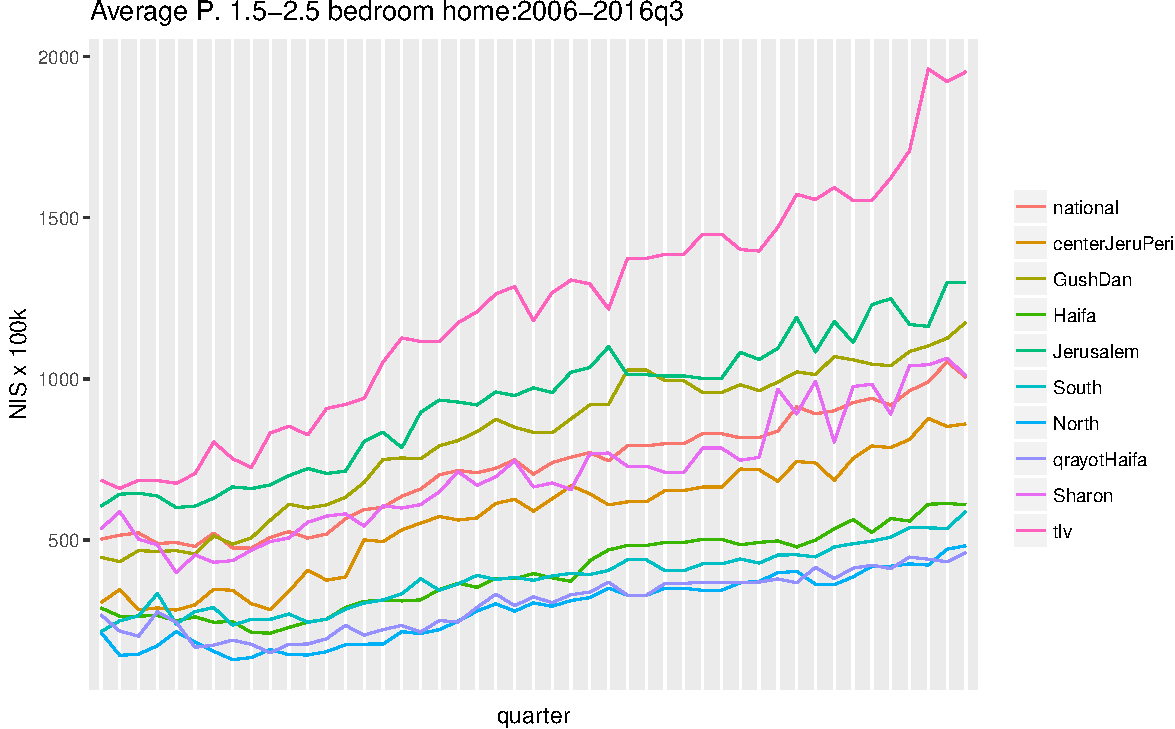
\includegraphics{publishedVersion_files/figure-latex/FigureOne-1.pdf}
\caption{\label{fig:FigureOne}I wrote this.}
\end{figure}

Consider the pretty data plotted in Figure \ref{fig:FigureOne}.

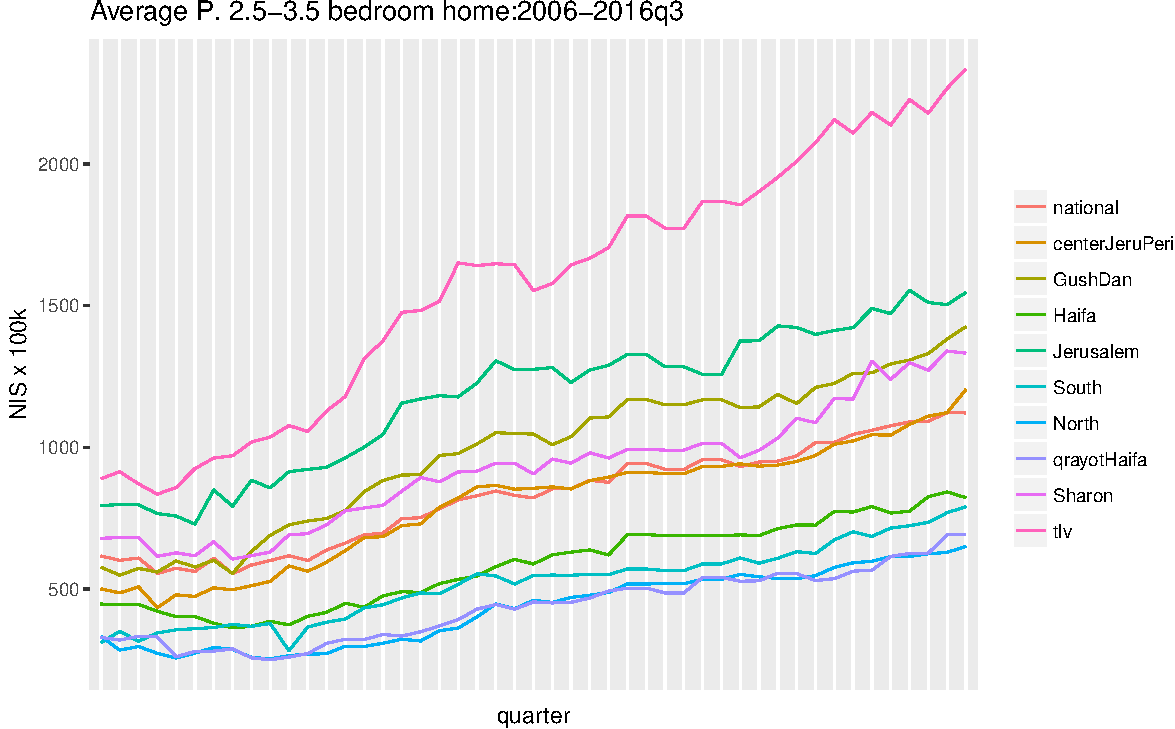
\includegraphics{publishedVersion_files/figure-latex/unnamed-chunk-1-1.pdf}
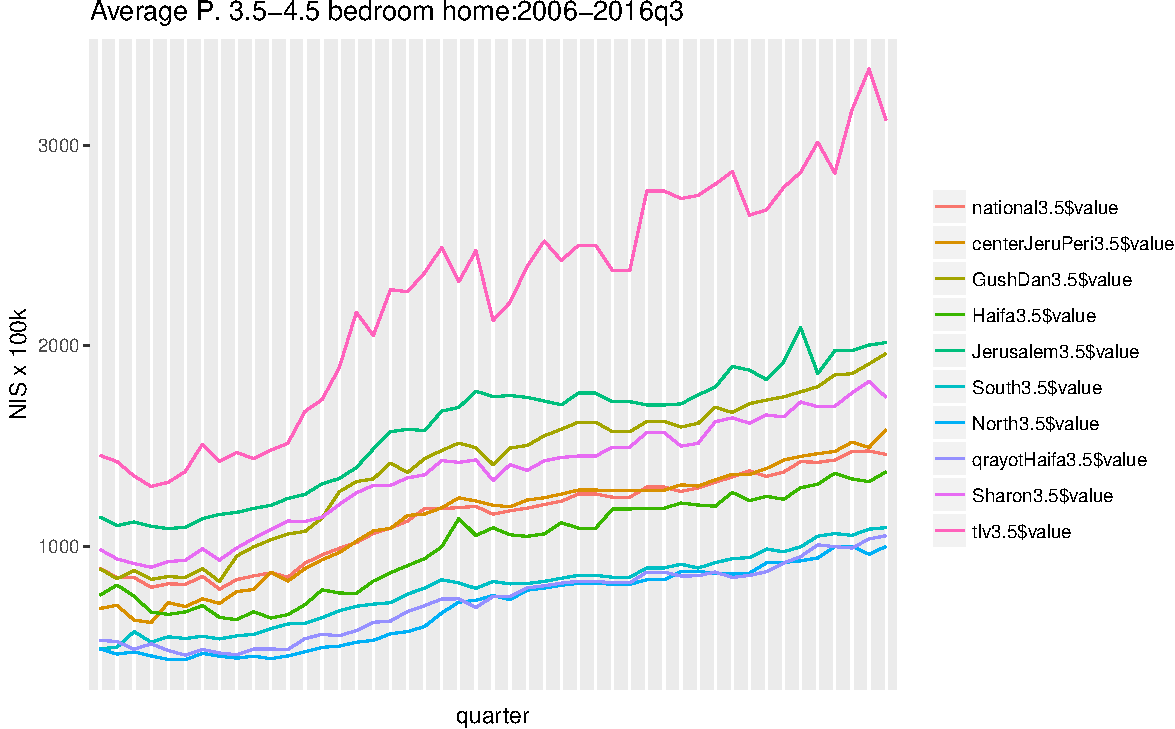
\includegraphics{publishedVersion_files/figure-latex/unnamed-chunk-1-2.pdf}
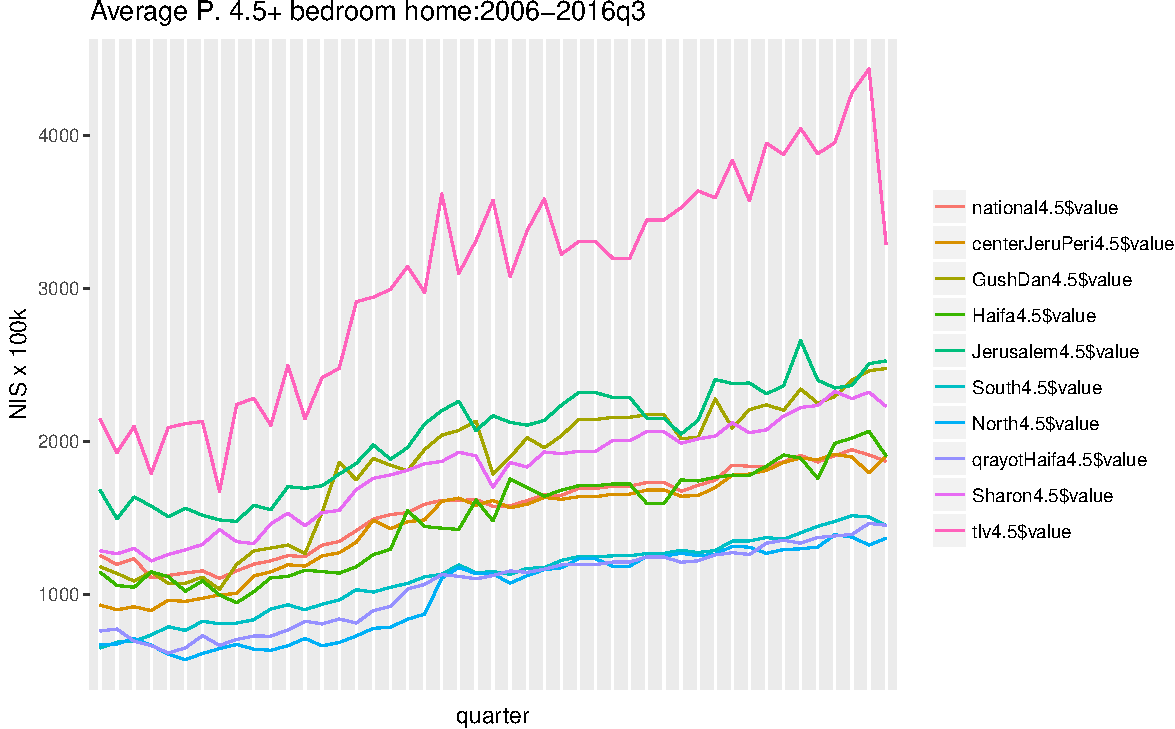
\includegraphics{publishedVersion_files/figure-latex/unnamed-chunk-1-3.pdf}

\printbibliography


\end{document}
